% Auto-generated by experiments.analysis.generate_ci_plots --- do not edit.
\begin{figure}[H]
\centering
\adjustbox{max width=\textwidth}{%
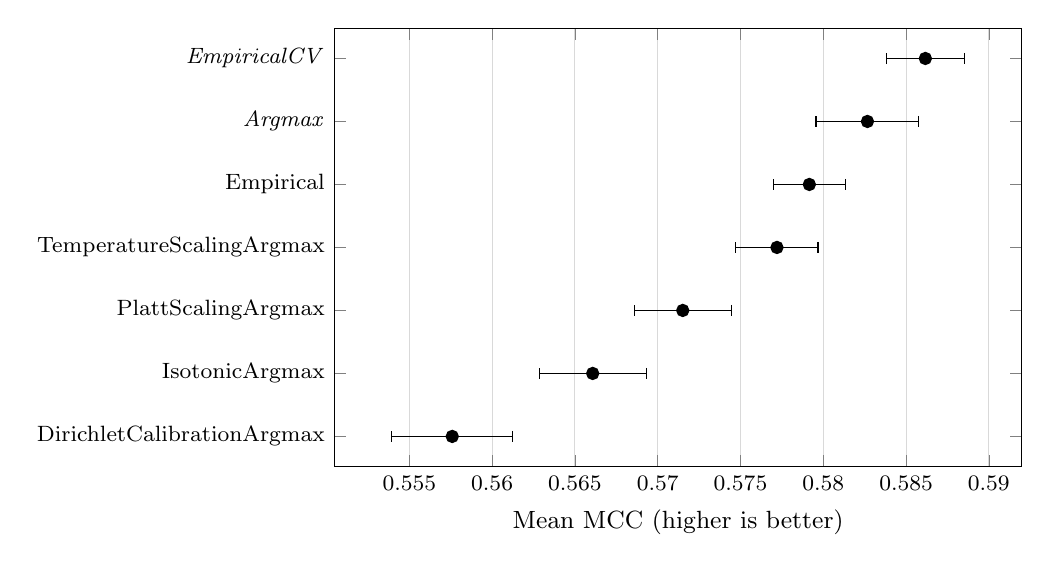
\begin{tikzpicture}
\begin{axis}[
    width=0.85\textwidth, height=7.15cm,
    xlabel={Mean MCC (higher is better)},
    symbolic y coords={{EmpiricalCV},{Argmax},{Empirical},{TemperatureScalingArgmax},{PlattScalingArgmax},{IsotonicArgmax},{DirichletCalibrationArgmax}},
    ytick={{EmpiricalCV},{Argmax},{Empirical},{TemperatureScalingArgmax},{PlattScalingArgmax},{IsotonicArgmax},{DirichletCalibrationArgmax}},
    yticklabels={\textit{EmpiricalCV},\textit{Argmax},Empirical,TemperatureScalingArgmax,PlattScalingArgmax,IsotonicArgmax,DirichletCalibrationArgmax},
    y dir=reverse,
    enlarge y limits=0.08,
    xmajorgrids=true,
    major grid style={draw=black!15, line width=0.3pt},
    scaled x ticks=false,
    xticklabel style={/pgf/number format/fixed, /pgf/number format/precision=3},
    tick label style={font=\footnotesize},
    label style={font=\small},
    every axis plot/.append style={thick},
]
\addplot[only marks, mark=*, mark size=2pt, color=black, error bars/x dir=both, error bars/x explicit, error bars/error bar style={color=black, line width=0.5pt}] coordinates { (0.586167,{EmpiricalCV}) +- (0.00235058,0) };
\addplot[only marks, mark=*, mark size=2pt, color=black, error bars/x dir=both, error bars/x explicit, error bars/error bar style={color=black, line width=0.5pt}] coordinates { (0.582668,{Argmax}) +- (0.00310402,0) };
\addplot[only marks, mark=*, mark size=2pt, color=black, error bars/x dir=both, error bars/x explicit, error bars/error bar style={color=black, line width=0.5pt}] coordinates { (0.57916,{Empirical}) +- (0.00218688,0) };
\addplot[only marks, mark=*, mark size=2pt, color=black, error bars/x dir=both, error bars/x explicit, error bars/error bar style={color=black, line width=0.5pt}] coordinates { (0.577204,{TemperatureScalingArgmax}) +- (0.00247722,0) };
\addplot[only marks, mark=*, mark size=2pt, color=black, error bars/x dir=both, error bars/x explicit, error bars/error bar style={color=black, line width=0.5pt}] coordinates { (0.571515,{PlattScalingArgmax}) +- (0.00292098,0) };
\addplot[only marks, mark=*, mark size=2pt, color=black, error bars/x dir=both, error bars/x explicit, error bars/error bar style={color=black, line width=0.5pt}] coordinates { (0.566076,{IsotonicArgmax}) +- (0.00322504,0) };
\addplot[only marks, mark=*, mark size=2pt, color=black, error bars/x dir=both, error bars/x explicit, error bars/error bar style={color=black, line width=0.5pt}] coordinates { (0.557592,{DirichletCalibrationArgmax}) +- (0.00365129,0) };
\end{axis}
\end{tikzpicture}%
}
\caption{adult: MCC on TabM (higher is better). Each dot is a strategy's mean over ten seeds with a $\pm 1$ SE horizontal bar; rows are sorted by mean, and the best strategy and any whose interval overlaps it are italicized.}%
\label{fig:ci-adult-mcc}
\end{figure}
